
In this chapter, it is presented results and discussions on numerical simulation of the experiment of \cite{chen} using the methodology introduced in the preceding chapters. The first section shows results of spread rate and self-similar profiles of the gas phase turbulent jet. The second section shows results of droplet and gas velocities and droplet dispersion. The third section presents liquid mass flow rates, vapor mass fluxes and droplet Sauter mean diameter.

\section{The Turbulent Round jet}

Consider the following definitions for the turbulent round jet:
\begin{description}
 \item[Jet half-radius ($y_{1/2}(x)$):] the radial coordinate for which the mean axial velocity is half of the mean axial velocity at the centerline for some axial coordinate $x$:
\begin{equation}
\tilde{U}_x (y=y_{1/2}) = \frac{1}{2}\tilde{U}_x(y=0) \, .
\end{equation}
\item[Dimensionless radial coordinate ($\hat{y}(x,y)$):]
\begin{equation}
 \hat{y} = \frac{y}{y_{1/2}} \, .
\end{equation}

\item[Dimensionless Mean Axial Velocity ($\hat{U}$):]
\begin{equation}
 \hat{U} = \frac{\tilde{U}_x-\tilde{U}_{\text{co-flow}}}{\tilde{U}_x (y=0)-\tilde{U}_{\text{co-flow}}} \, ,
\end{equation}
where $\tilde{U}_{\text{co-flow}}$ is the mean axial velocity of the co-flow stream specified in the boundary condition.

\item[Dimensionless Turbulent Kinetic Energy $\hat{k}$:]
\begin{equation}
 \hat{k}=\frac{k}{(\tilde{U}_x (y=0)-\tilde{U}_{\text{co-flow}})^2} \, .
\end{equation}

\item[Dimensionless Turbulent Viscosity ($\hat{\nu}_T$):]
\begin{equation}
\hat{\nu}_T = \frac{\mu}{\bar{\rho}\tilde{U}_x(y=0) y_{1/2}} \, .
\end{equation}

\item[Jet Spread Rate ($S$):]
\begin{equation}
S = \frac{d y_{1/2} (x)}{dx} \, .
\end{equation}
\end{description}

An empirical observation of a gas turbulent round jet is that the profiles of $\hat{U}$, $\hat{k}$ and $\hat{\nu}_T$ as function of $\hat{y}$ becomes self-similar (i.e. independent of the axial coordinate) from some distance to the nozzle exit.
Furthermore, there is a linear relation between the half-radius ($y_{1/2}$) and the axial coordinate, that is, the jet sprad rate is constant.

\cite{chen} has experimentally shown that self-similarity also occurred for $\hat{U}$ in the presence of the spray jet for $x/D \ge 10$. For arriving at this conclusion, it assumed the velocity measured for the smaller droplets ($D<3\mu m$) as being the gas velocity. 

The group of Figures \ref{fig: selfsimilar_profile} shows the same investigation for the gas velocity field obtained in the numerical simulation. The Figure \ref{ssA} shows the profiles of $\hat{U}$ for several axial coordinates. Differently than the experiment, the self-similarity only occurs for $x/D \ge 15$ (and not for $x/D \ge 10$). This suggests that the transition from the jet developing region to the turbulent region is retarded in the simulation.

\begin{notation}
$<f''>$ or $<f'>$ denotes the root mean square of the fluctuation $f''$ (for a Favre average) or $f'$ (for a time average).
\end{notation}

Figures \ref{ssB} and \ref{ssC} show that the evolution to self-similar profiles is slower for the turbulent quantities $\hat{k}$ and $\hat{\nu}_T$ and one may not say that the self-similarity was achieved inside the domain. \cite{chen} has shown that for $x/D \le 25$ it was also not achieved in the experiment for the root mean square of the axial velocity fluctuation ($<U''_x>$). 

One observation concerning the turbulent viscosity ($\hat{\nu}_T$) is that the centerline value seems to evolve to a value of $\hat{\nu}_T = 0.047$, higher than values found in the literature for the turbulent round jet. \cite{pope2000turbulent} reports a self-similar turbulent viscosity at centerline of $\hat{\nu}_T = 0.029$.


\begin{figure}[!htb]
 \centering
\begin{tabular}{c}
 \subfloat[]{\label{ssA}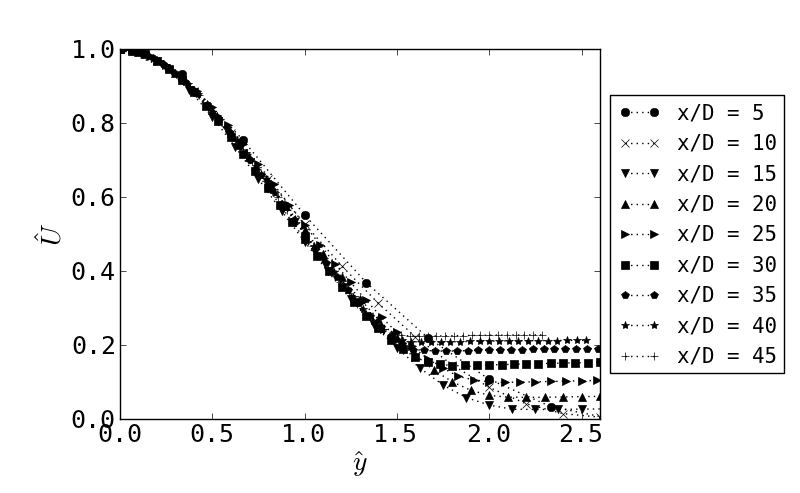
\includegraphics[width=0.65\textwidth]{./figuras/chap5/selfsimilar/selfsimilar_U.png}} \\
 \subfloat[]{\label{ssB}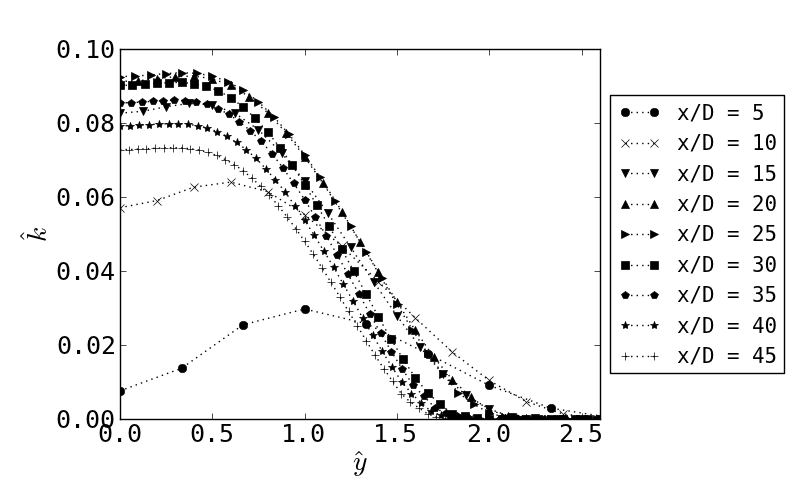
\includegraphics[width=0.65\textwidth]{./figuras/chap5/selfsimilar/selfsimilar_k.png}} \\
 \subfloat[]{\label{ssC}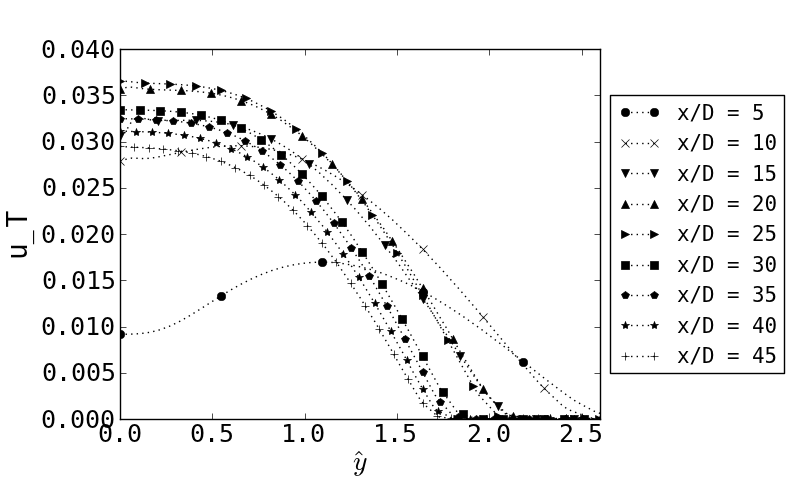
\includegraphics[width=0.65\textwidth]{./figuras/chap5/selfsimilar/selfsimilar_nut.png}} \\
\end{tabular}
 \caption{Numerical results showing the evolution to self-similar profiles of the following gas phase properties: (a) dimensionless mean axial velocity - $\hat{U}_x$, (b) dimensionless turbulent kinetic energy - $\hat{k}$ - and (c) dimensionless turbulent viscosity - $\hat{\nu}_t$. The different curves show the profiles for the corresponding axial coordinate indicated in the legend.}
\label{fig: selfsimilar_profile}
\end{figure}

The jet spread rate measures the spread of the axial velocity in the radial direction. A value about $S=0.095$ is found on the literature for the pure gas flow \cite{pope2000turbulent}, and it is independent of Reynolds number. For the spray jet, however, \cite{chen} has reported $S=0.066$. In the simulation, it was found a higher value of $S=0.071$, a difference of $23\%$. 

The Figure \ref{fig: ssS} shows the indeed different half-radius values found in the simulation and the experiment for the same axial coordinates, and Figure \ref{fig: ssP} compares the self-similar profiles of $\hat{U}_x$ from the simulation and the experiment.

The overestimation of the round jet spread rate with the default coefficients of k-epsilon turbulence model has been reported previously by different authors. \cite{luppes} has discussed four alternatives to the correction. The modifications consist not only in changing the model coefficients, but also tunning of boundary conditions. 

No correction was used in this work because the exact modifications are not known in advance. The effect of this discrepancy on the droplet velocities is discussed in the next section. 

\begin{figure}[!htb]
 \centering
\begin{tabular}{cc}
 \subfloat[]{\label{fig: ssS}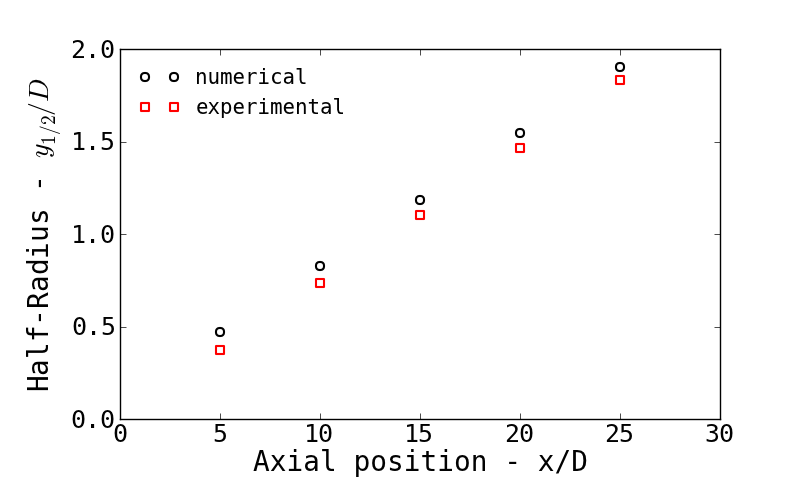
\includegraphics[width=0.5\textwidth]{./figuras/chap5/selfsimilar/selfsimilar_spread.png}} & \subfloat[]{\label{fig: ssP}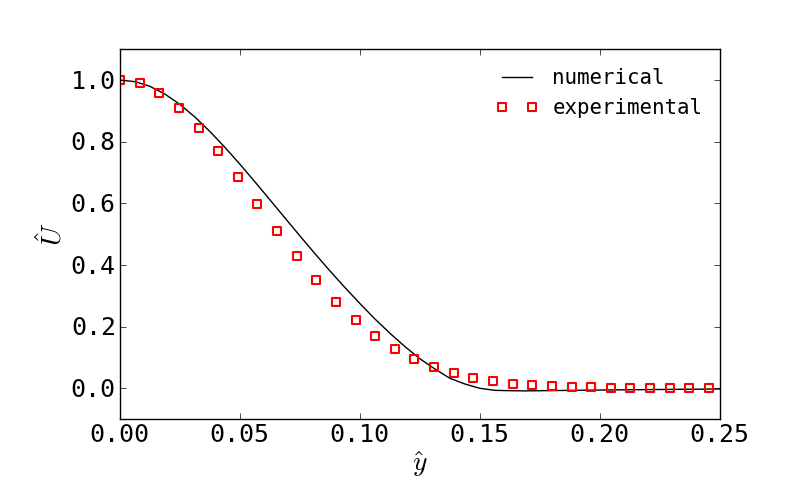
\includegraphics[width=0.5\textwidth]{./figuras/chap5/selfsimilar/selfsimilar_num_exp.png}}
\end{tabular}
 \caption{(a) Half-radius as a function of the axial coordinate in the experiment and in the simulation.  (b) Self-similar radial profile of the numerical and the experimental dimensionless axial velocity - $\hat{U}_x$. The measurements were obtained from \cite{chen}.}
\label{fig: selfsimilar_spread}
\end{figure}

\FloatBarrier
\section{Gas and Droplet Velocities and Droplet Dispersion}

\cite{chen} has presented velocity measurements for droplets of four diameter classes in the spray jet: $D< 5\mu m$, $10\mu m <D<20\mu m$, $20 \mu m < D < 30 \mu m$ and $30 \mu m < D < 40 \mu m$. The importance of separating the data in droplet size classes is that the drag force is dependent on its size. 

Figure \ref{fig: drop_drag} shows the time response to drag force as modeled in Equation \eqref{eq: drop_dudt} for droplets with diameter ranging from $10$ to $40\mu m$ and initial velocity of $10\ m/s$. The time for the droplet with diameter of $40\ \mu m$ comes to rest is nearly $10$ times greater than the required for the droplet with $10\ \mu m$.

\begin{figure}
 \centering
\begin{tabular}{c}
 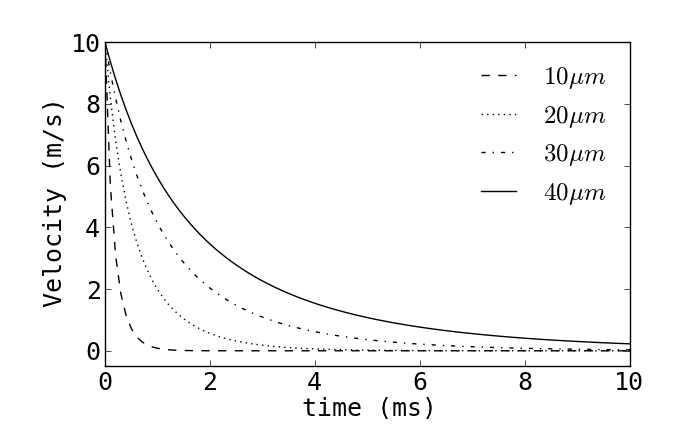
\includegraphics[width=0.65\textwidth]{./figuras/chap5/drag/drop_drag.png}
\end{tabular}
 \caption{Solution of droplet drag model of Equation \eqref{eq: drop_dudt}. Droplet velocity as a function of time for an initial velocity of $10\ m/s$ in stagnant air at standard conditions and for droplet diameters of $10$, $20$, $30$ and $40 \mu m$. }
 \label{fig: drop_drag}
\end{figure}

% The calculation accuracy of the droplet dispersion is mainly dependent on how much of gas turbulence is resolved and the droplets Stoke number. Higher Stokes numbers ($St \ge 10$) allow less resolution of flow turbulence because droplet is more likely to follow the mean velocity field. 

This fast response of smaller droplets provides a good estimative of the gas velocity. \cite{chen} has measured the velocity of droplets with $D< 5\ \mu m$ that here will be assumed to represent also the experimental gas velocity. The consequences of the larger spread rate mentioned before may then be evaluated directly in the radial profile of the mean axial velocity.

Figure \ref{fig: Ux_gas} shows in red squares the measured radial profiles of the mean axial velocity for the gas phase ($\tilde{U}_x$) in the axial coordinates of: $x/D=5$, $10$, $15$, $20$ and $25$. The radial profile obtained in the simulation is also shown in a solid black line. It is evident that the underprediction of the gas velocity in the simulation becomes higher in the downstream direction. In the axial coordinate of $x/D=25$, the centerline value in the simulation is about $20\%$ below the experimental value.

\begin{figure}[!htb]
 \centering
\begin{tabular}{cc}
 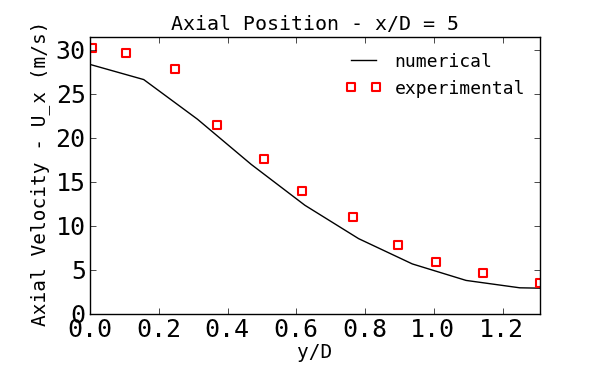
\includegraphics[width=0.5\textwidth]{./figuras/chap5/Ux/Ux_gas/Ux_gas5.png} & 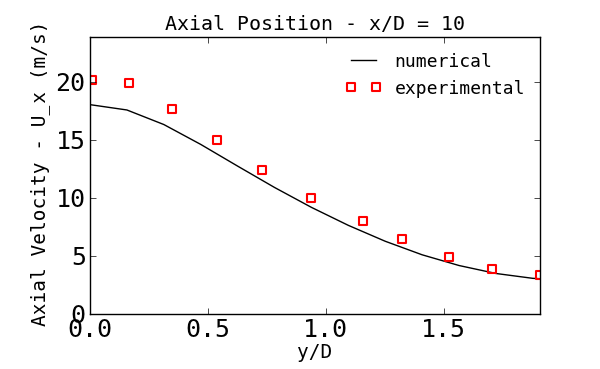
\includegraphics[width=0.5\textwidth]{./figuras/chap5/Ux/Ux_gas/Ux_gas10.png} \\
(a) & (b) \\
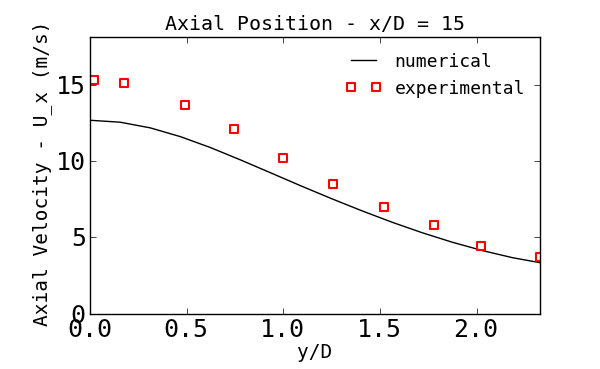
\includegraphics[width=0.5\textwidth]{./figuras/chap5/Ux/Ux_gas/Ux_gas15.png} & 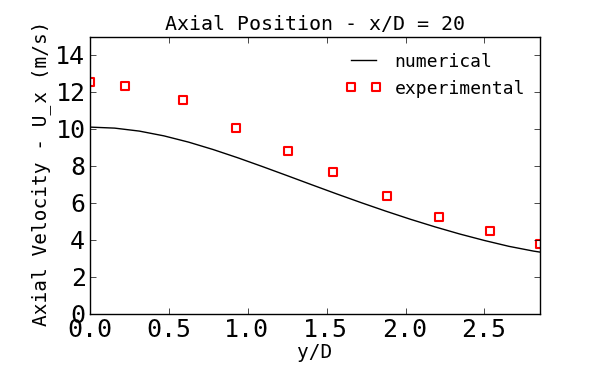
\includegraphics[width=0.5\textwidth]{./figuras/chap5/Ux/Ux_gas/Ux_gas20.png} \\
(c) & (d) \\
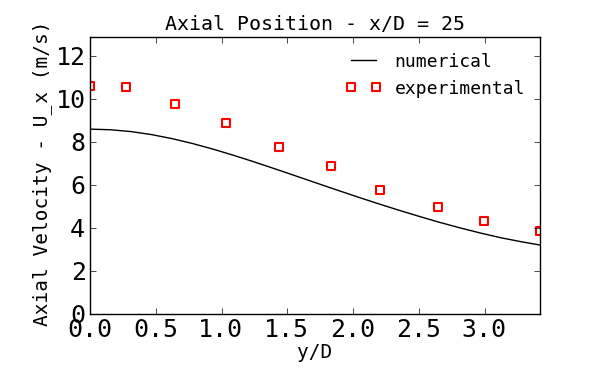
\includegraphics[width=0.5\textwidth]{./figuras/chap5/Ux/Ux_gas/Ux_gas25.png} &   \\
(e) & \\
\end{tabular}
 \caption{Measured and computed radial profiles of the mean axial velocity of the gas phase ($\tilde{U}_x$). Each figure shows the profile in a different axial location: $x/D=5$ in (a), $x/D=10$ in (b), $x/D=15$ in (c), $x/D=20$ in (d) and $x/D=25$ in (e). The measurements were obtained from \cite{chen}.}
 \label{fig: Ux_gas}
\end{figure}

It may be questioned whether the flux of gas momentum in the nozzle exit were correct because the gas exiting temperature was estimated from an assumption of thermal equilibrium with the liquid phase, as explained in Equation \eqref{eq: bc_est_T} in Chapter \ref{chap: exp}. If temperature were lower than in the experiment, then the density and the momentum flux would also be lower.

However, that was not the case. Velocity agreement was good, see Figure \ref{fig: bc_Ux}, and nozzle mass flow rate matches measurements within $1.5\%$. This led to the conclusion that the momentum flux was correctly specified in the nozzle exit and that the discrepancies in velocity were due only to the turbulence modeling.

In fact, \cite{luppes} has reported an error of the same percentual magnitude using the k-epsilon model with the default coefficients. This result is reproduced in Figure \ref{fig: luppes}. The simulation with default k-epsilon coefficients is represented as the curve \textit{simulation 1}. The others curves are results obtained by tunning the model parameters and the boundary conditions.

\begin{figure}[!htb]
 \centering
\begin{tabular}{c}
 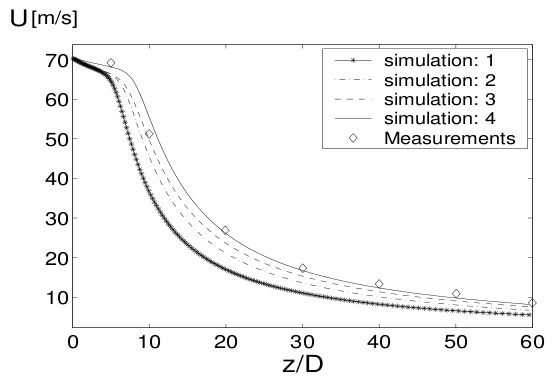
\includegraphics[width=0.6\textwidth]{./figuras/chap5/refs/luppes_vel.png} 
\end{tabular}
 \caption{The comparison of four simulations of a turbulent air jet (Re = 37,600) with measurements. The centerline axial velocity is shown. In each plot the axial distance is normalized by the nozzle diameter. Simulation 1:
standard k-epsilon model. Simulation 2: $c_{\mu} =0.06$. Simulation 3: $c_{\mu}=0.06$, $c_{\epsilon, 2} =1.87$. Simulation 4: $c_{\mu}=0.09$, $c_{\epsilon, 2}=1.87$, n =10. Figure reproduced from \cite{luppes}.}
 \label{fig: luppes}
\end{figure}

 \cite{chen} has also reported the root mean square of axial and radial velocities, respectively $<U''_x>$ and $<U''_y>$. Again, the values for the smaller droplets ($D< 5\ \mu m$) are being used to represent the gas velocity. The same quantities are not provided in the simulation for direct comparison. The turbulence model only solves for the turbulent kinetic energy and its dissipation rate. A characteristic velocity, however, may be defined as $<U''>=\sqrt{2/3 k}$. This quantity is shown in Figure \ref{fig: UUx} with $<U''_x>$ and $<U''_y>$. Again, it is shown radial profiles for different axial coordinates.

Three observations are readily made:  
\begin{itemize}
  \item The radial profile of $<U''_x>$ is similar to that of $<U''_y>$;
  \item The characteristic velocity defined for the k-epsilon model ($<U''>$) agrees well with $<U''_x>$ and $<U''_y>$;
 \item $<U''>$ declines faster than $<U''_x>$ and $<U''_y>$ as the axial coordinate increases.
\end{itemize}

The first observation indicates that the turbulent jet differs from the self-similar profiles found in the literature \cite{pope2000turbulent}, where $<U''_x>$ is about twice as big as $<U''_y>$ in the centerline. It remains the question whether this occurs because the jet is not fully developed or because of some spray influence.

The second observation suggests that the k-epsilon model is appropriate to describe the round jet turbulence, providing an appropriate characteristic velocity. The third observation, however, indicates that the turbulent dissipation is overpredicted.

\begin{figure}[!htb]
 \centering
\begin{tabular}{cc}
 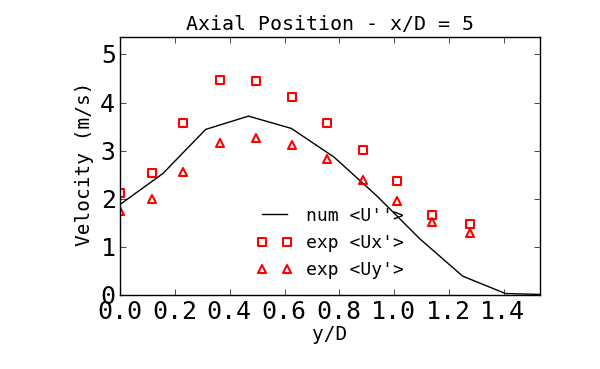
\includegraphics[width=0.5\textwidth]{./figuras/chap5/UU/UUx5.png} & 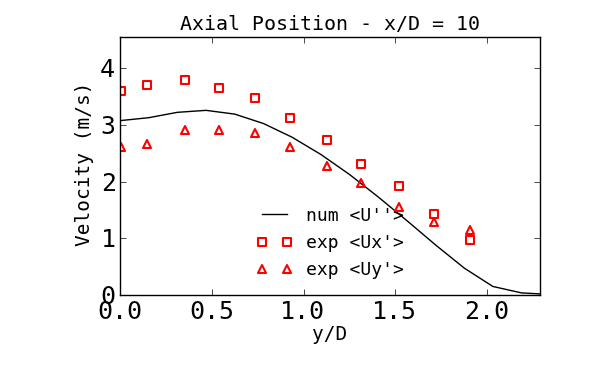
\includegraphics[width=0.5\textwidth]{./figuras/chap5/UU/UUx10.png} \\
(a) & (b) \\
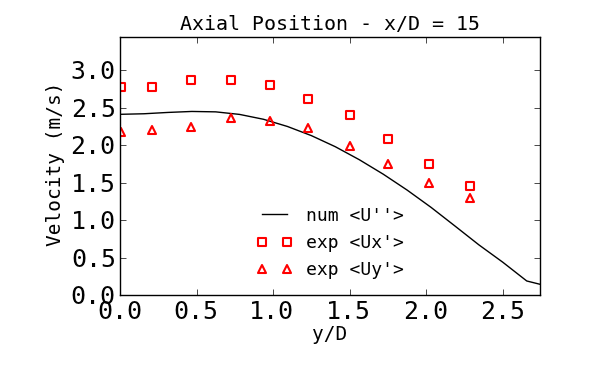
\includegraphics[width=0.5\textwidth]{./figuras/chap5/UU/UUx15.png} & 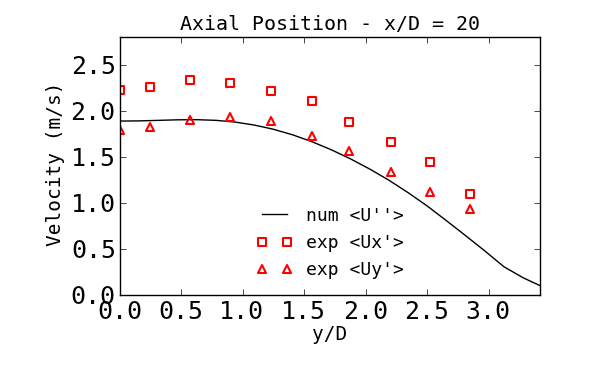
\includegraphics[width=0.5\textwidth]{./figuras/chap5/UU/UUx20.png} \\
(c) & (d) \\
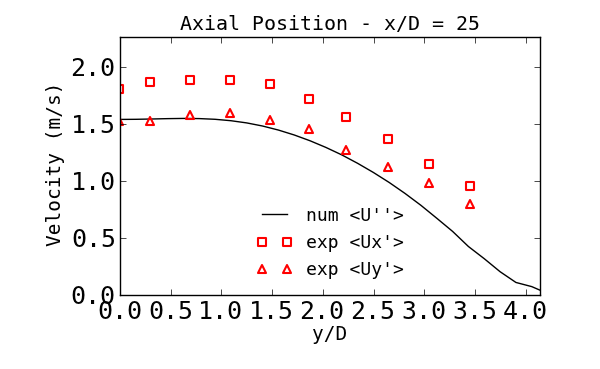
\includegraphics[width=0.5\textwidth]{./figuras/chap5/UU/UUx25.png} &  \\
(e) & \\
\end{tabular}
 \caption{Measured radial profiles of the gas phase velocities $<U''_x>$ and $<U''_y>$ and the characteristic velocity defined for the k-epsilon model $<U''>=\sqrt{2/3 k}$ obtained from the simulation. Each figure shows the profile in a different axial location: $x/D=5$ in (a), $x/D=10$ in (b), $x/D=15$ in (c), $x/D=20$ in (d) and $x/D=25$ in (e). The measurements were obtained from \cite{chen}.}
\label{fig: UUx}
\end{figure}

Returning to the mentioned influence of the discrepancies in the mean axial velocity of the gas phase on the droplet velocities, the lower velocity of the gas increases the droplet slip velocity and causes a larger drag to be felt by them. The obvious conclusion is that the same discrepancy in the gas velocity will be observed in the comparison of experimental and numerical values of the droplet velocities.

Figure \ref{fig: Ux} shows in red squares the radial velocity profile measured  by \cite{chen} for droplets in the class of $10\mu m <D<20\mu m$ in the axial coordinates of: $x/D=5$, $10$, $15$, $20$ and $25$.  For each radial position, the velocity value is the ensemble average of the droplets crossing the laser PDI beams. The droplet velocity obtained in the simulation is also shown as black scattered points representing each of them a different droplet in the computation, no averaging was performed.

It is observed that the computed droplet velocity also becomes systematically lower than the measurements in the downstream direction.

\begin{figure}[!htb]
 \centering
\begin{tabular}{cc}
 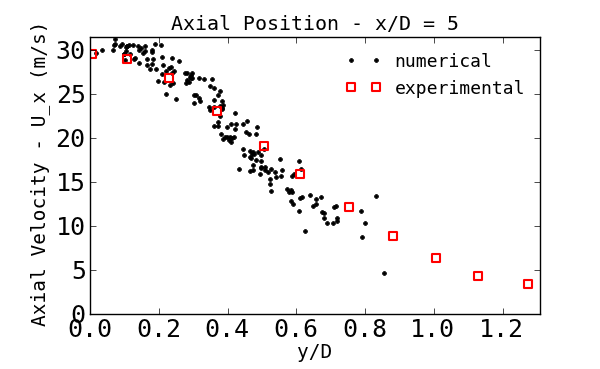
\includegraphics[width=0.5\textwidth]{./figuras/chap5/Ux/Ux_drops/Ux_x5.png} & 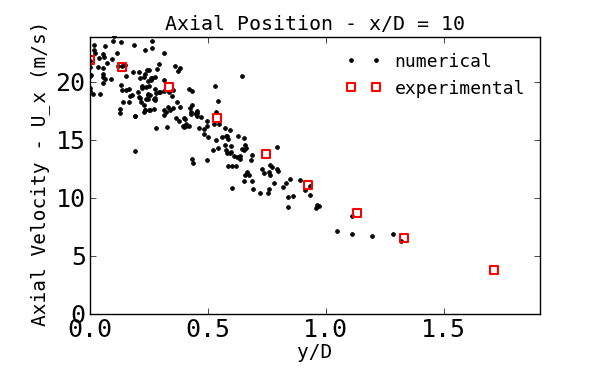
\includegraphics[width=0.5\textwidth]{./figuras/chap5/Ux/Ux_drops/Ux_x10.png} \\
(a) & (b) \\
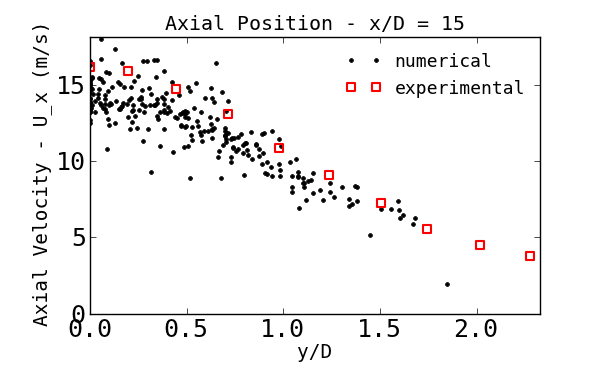
\includegraphics[width=0.5\textwidth]{./figuras/chap5/Ux/Ux_drops/Ux_x15.png} & 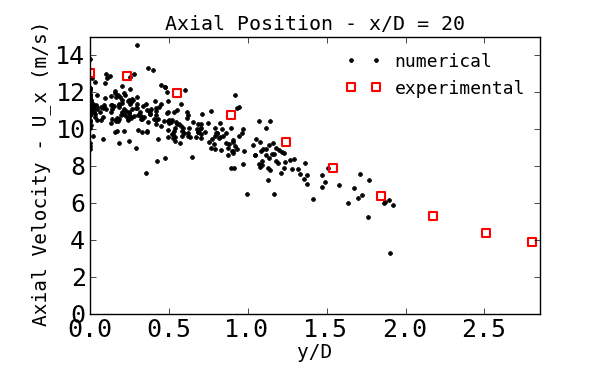
\includegraphics[width=0.5\textwidth]{./figuras/chap5/Ux/Ux_drops/Ux_x20.png} \\
(c) & (d) \\
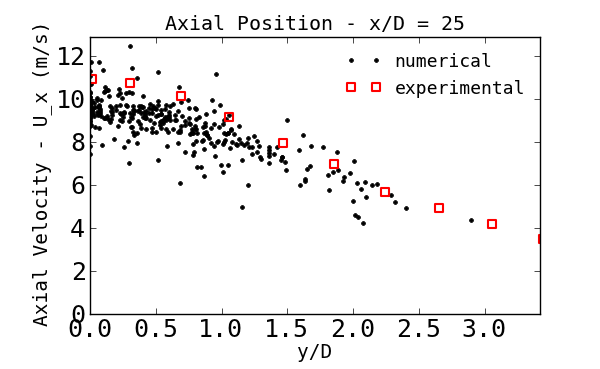
\includegraphics[width=0.5\textwidth]{./figuras/chap5/Ux/Ux_drops/Ux_x25.png} &   \\
(e) & \\
\end{tabular}
 \caption{Red squares present measured radial profiles of mean axial velocity of droplets ($\tilde{U}_{d,x}$) in the size class of $10\mu m <D<20\mu m$. Scattered black dots are the computed velocities for each droplet in the numerical simulation. Each figure shows the velocity profile in the axial coordinate specified above the plot window. The measurements were obtained from \cite{chen}.}
 \label{fig: Ux}
\end{figure}

The last result concerning the droplet velocity is the droplet dispersion: the differences in droplet velocities found in different size classes. Figure \ref{fig: jointUV} shows the numerical instantaneous radial velocity ($U_{y}$) as function of radial coordinate for two extreme size classes: $D< 10\ \mu m$ and $D> 30\ \mu m$. It is seen that the smaller droplets are more sensitive to the gas velocity sampled in the turbulent dispersion model introduced in Chapter \ref{chap: equations}, specially near the nozzle exit. The biggest droplets show a smaller dispersion around the zero mean value because of their higher inertia. As the axial coordinate increases, both behaviors become similar.

\begin{figure}[!htb]
 \centering
\begin{tabular}{cc}
 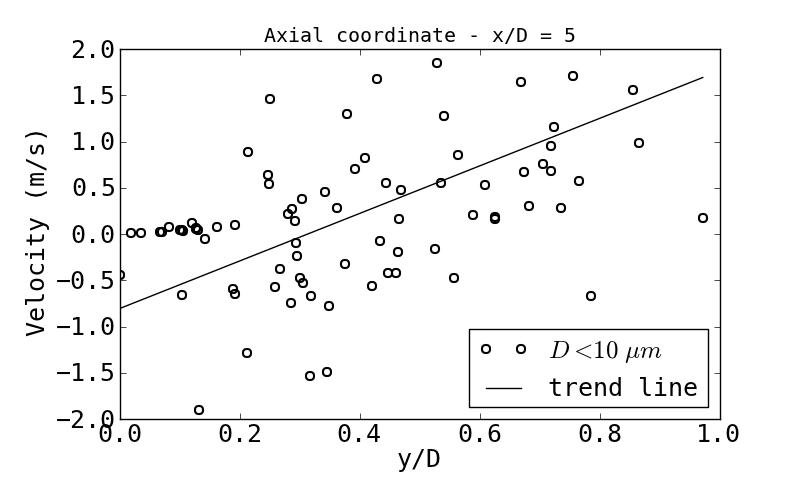
\includegraphics[width=0.5\textwidth]{./figuras/chap5/dispersion/class0_5.png} & 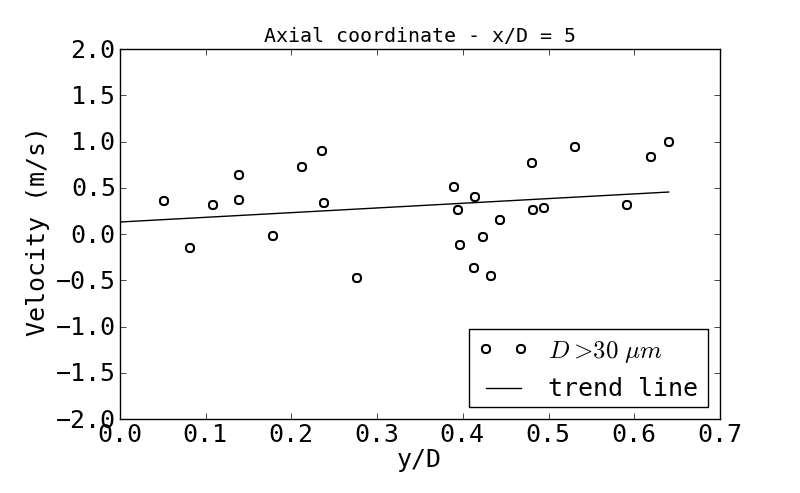
\includegraphics[width=0.5\textwidth]{./figuras/chap5/dispersion/class4_5.png} \\
(a) & (b) \\
 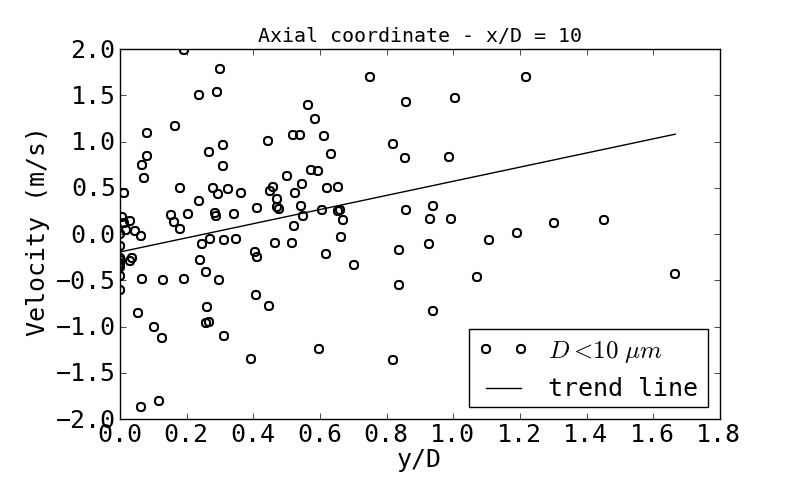
\includegraphics[width=0.5\textwidth]{./figuras/chap5/dispersion/class0_10.png} & 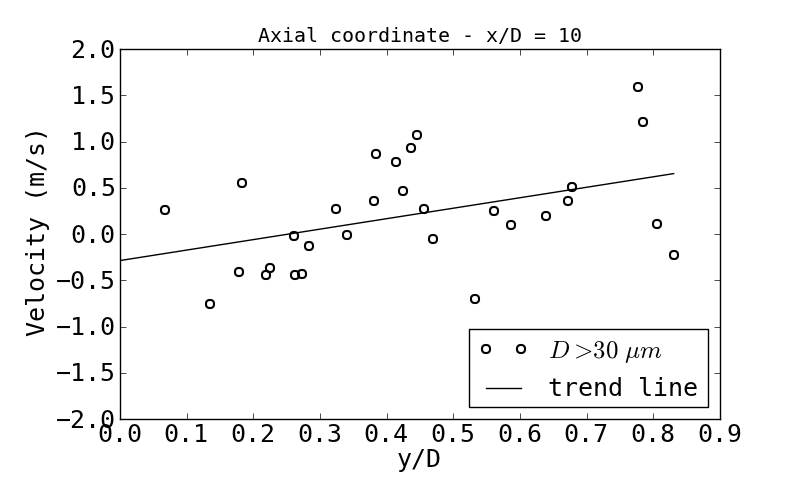
\includegraphics[width=0.5\textwidth]{./figuras/chap5/dispersion/class4_10.png} \\
(c) & (d) \\
 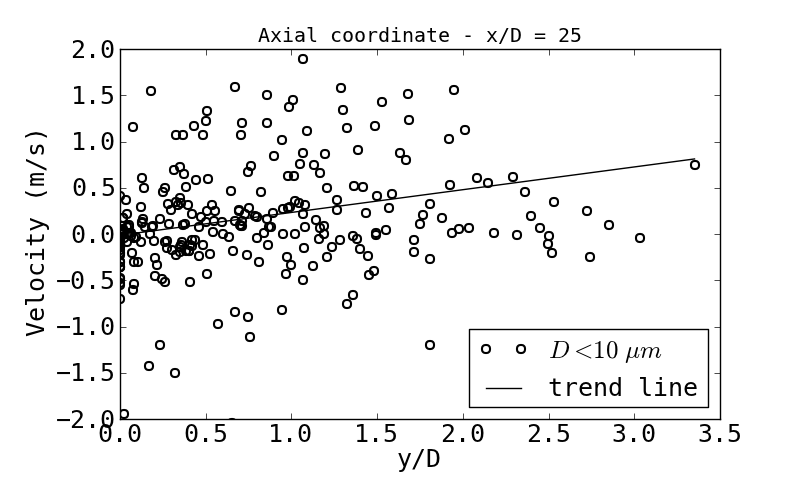
\includegraphics[width=0.5\textwidth]{./figuras/chap5/dispersion/class0_25.png} & 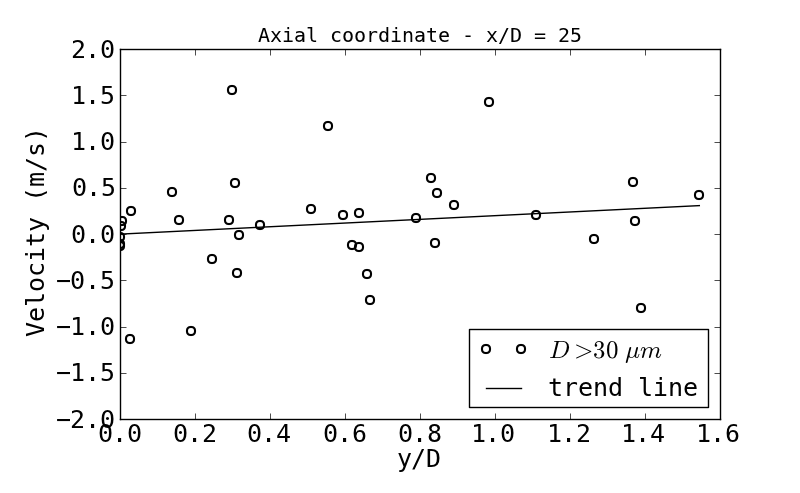
\includegraphics[width=0.5\textwidth]{./figuras/chap5/dispersion/class4_25.png} \\
(e) & (f)
\end{tabular}
 \caption{Scatter plot of the numerical radial velocity of droplets ($U_{y}$) in two different size classes: $D< 10\ \mu m$ on the left or (a), (c) and (e) labels; and $D> 30\ \mu m$ on the right or (b), (d) and (f) labels. The dispersion in the radial velocity is higher for the smaller droplet class and in the vicinity of the nozzle exit.}
\label{fig: jointUV}
\end{figure}

\FloatBarrier
\section{Liquid Mass Flow Rate and Vapor Mass Fluxes}

Correct prediction of droplet evaporation is, together with velocity, of high importance for applications of spray simulation. Reasonably low discrepancies found for droplet velocity in Figure \ref{fig: Ux} already indicates that the evaporation model performed well. This is due to the fact that an incorrect modeling of evaporation would lead to an erroneous droplet diameter, further affecting velocity prediction.

Figure \ref{fig: droplet_flux} shows numerical and experimental liquid mass flow rate for different axial coordinates. Computed values are in good agreement with measurements for $x/D \le 10$. Further downstream, the simulation overpredicts the liquid flow rate. Clearly, this means that droplet evaporation is lower than it should be. In fact, in Figure \ref{fig: vapor_flux}, it is made the comparison of experimental and numerical radial profiles of vapor mass fluxes and the trend is exactly the same: as the axial coordinate increases, less vapor (hence more liquid) is present in simulation than in experiment.

\begin{figure}[!htb]
\centering
  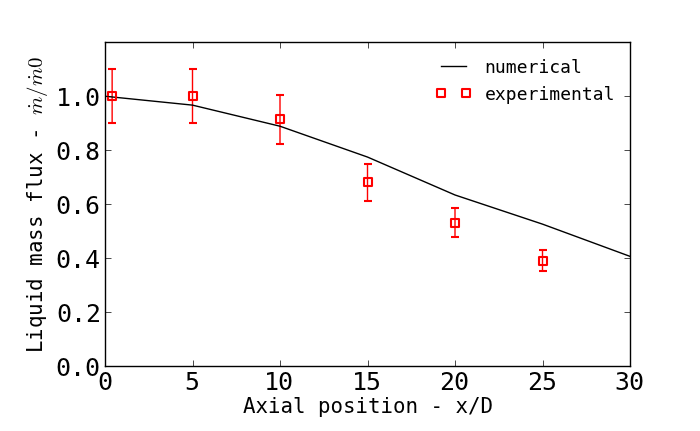
\includegraphics[width=0.6\textwidth]{./figuras/chap5/massflow/drop_mflux.png}
\caption{Droplet mass flow rate at four axial locations. Measurements were obtained from \cite{chen}.}
\label{fig: droplet_flux}
\end{figure} 


\begin{figure}[!htb]
 \centering
\begin{tabular}{cc}
 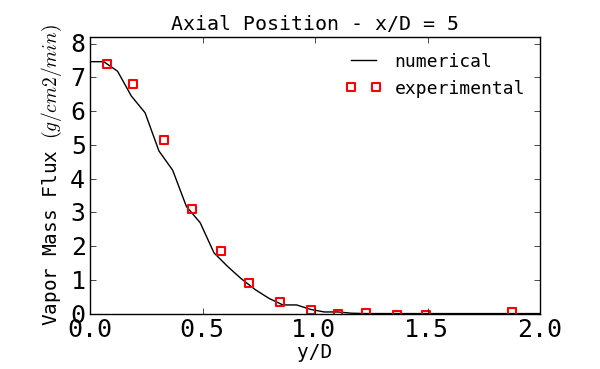
\includegraphics[width=0.45\textwidth]{./figuras/chap5/massflow/mvapor5.png} & 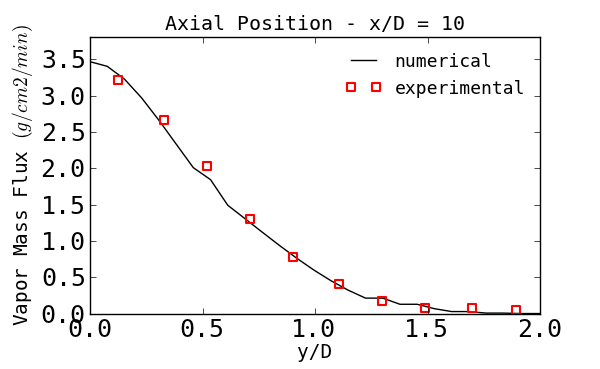
\includegraphics[width=0.45\textwidth]{./figuras/chap5/massflow/mvapor10.png} \\
(a) & (b) \\
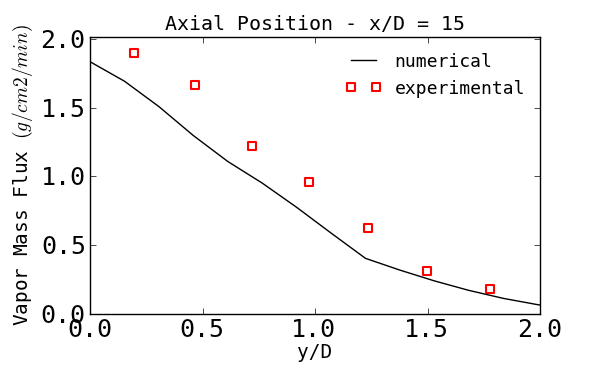
\includegraphics[width=0.45\textwidth]{./figuras/chap5/massflow/mvapor15.png} & 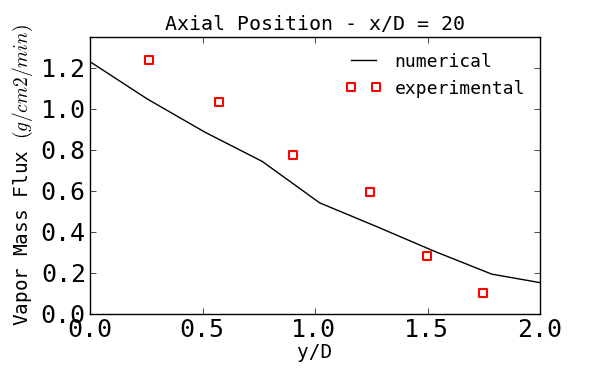
\includegraphics[width=0.45\textwidth]{./figuras/chap5/massflow/mvapor20.png} \\
(c) & (d)
\end{tabular}
 \caption{Radial profiles of mean axial mass flux of acetone vapor: $\dot{m}''_{ac}=\rho \bar{Y}_{ac} \tilde{U}_x$. The measurements were obtained from \cite{chen}.}
 \label{fig: vapor_flux}
\end{figure}

The underestimation of evaporation rate has also been noticed in a large-eddy simulation performed by \cite{bini}, where it was discussed the effect of a subgrid model to the evaporation. It is said that the lack of a subgrid model affects evaporation mainly in the jet core, where the mean vapor mass fraction might be saturated, but negative oscillations might allow for extra vaporization. In fact, the evaporation model presented in Chapter \ref{chap: equations} only deals with the averaged flow properties, and the temperature and mass fraction oscillations, ($T''$) and ($Y''_{ac}$), are not taken into account.

Surely, for a large-eddy simulation, the lack of a subgrid model is less severe than in RANS modeling since at least the non-filtered oscillations are present. 

A stochastic model for RANS simulation was proposed in \cite{santanu}. The proposed approach was to establish stochastic behaviors for $T''$ and $Y''_{ac}$ and use the instantaneous values of them ($T$ and $Y_{ac}$) in the heating and evaporation models. The results, however, did not improve significantly in the case it studied. This approach implies an odd assumption that the experimental correlations used for the droplet models, which were developed for a non-oscillating gas field, would work for an oscillating situation by only using instantaneous flow properties. A more profound discussion is found in \cite{sirignano}, where directly modeling of the Sherwood and the Nusselt numbers is suggested. This is the same approach used in \cite{bini} with good results.

It must also be pointed that uncertainties in the gas mean velocity also affect the droplet heating and evaporation prediction again because of the different slip velocity. The correct attempt to improve accuracy of the present computation would be to adjust the turbulence model to firstly correct the gas mean velocity and see the new evaporation rates. Next, a stochastic subgrid model for the heat and mass transfer coefficients could be studied.

\begin{figure}[!htb]
 \centering
\begin{tabular}{c}
 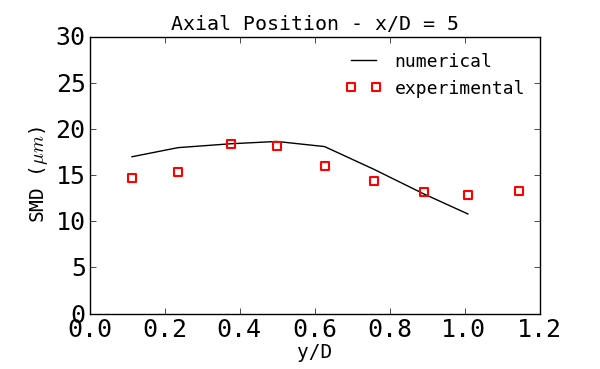
\includegraphics[width=0.5\textwidth]{./figuras/chap5/smd/smd5.png} \\
(a) \\
 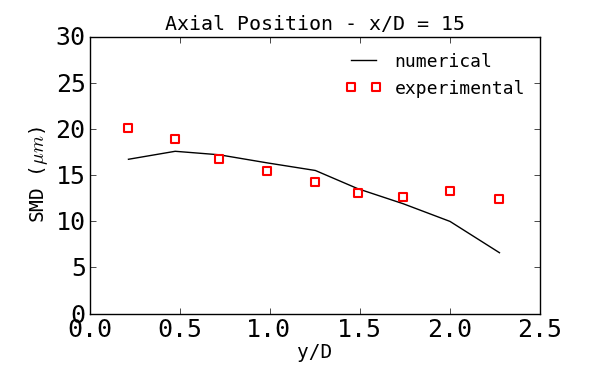
\includegraphics[width=0.5\textwidth]{./figuras/chap5/smd/smd15.png} \\
(b) \\
 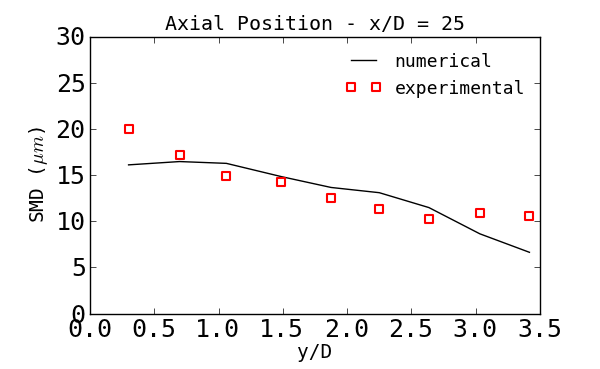
\includegraphics[width=0.5\textwidth]{./figuras/chap5/smd/smd25.png} \\
(c) 
\end{tabular}
 \caption{Numerical and experimental radial profiles of Sauter mean diameter (SMD). The measurements were obtained from \cite{chen}.}
 \label{fig: SMDprofile}
\end{figure}

The last studied property of the spray is the droplet Sauter mean diameter (SMD). Figure \ref{fig: SMDprofile} shows the numerical and experimental radial profiles of SMD.

The computed Sauter mean diameter shows a good agreement with measurements, in despite of the uncertainty about the droplet size distribution in the boundary conditions and the higher liquid flow rates in Figure \ref{fig: droplet_flux}. This may also be a consequence of the low variance in droplet diameter in the nozzle injection.

This agreement also confirms that the velocity discrepancy is caused by the anomalous jet spread rate. As discussed previously, if diameters were also in disagreement, the predicted drag force on the droplets would be further incorrect.


\FloatBarrier
